% !TeX spellcheck = hu_HU
% !TeX encoding = UTF-8
% !TeX program = xelatex
%----------------------------------------------------------------------------
\chapter{Használati példák}
%----------------------------------------------------------------------------

Ebben a fejezetben pár konkrét használati példát mutatok be a blAST eszközhöz.
A cél, hogy olyan felhasználási esetek legyenek, amelyeket valamilyen oknál fogva az általános eszközök, amelyeket \aref{ch:exist}.~fejezetben tárgyalt, nem, vagy nem kényelmesen tudnak kielégíteni.

\section{Kompatibilitási réteg}

Ha egy platformfüggetlen programot szeretne valaki csinálni, akkor könnyen belefut egy olyan szituációba, amelyikben olyan rendszer függvényt kell hívjon, amelyik nem könnyen hordozóható.
Egy példa lehet a memória lapozó függvények amelyiken {\tt mmap} néven elérhető POSIX rendszereken, míg {\tt MapViewOfFile} a Win32 alatti megfelelője.
De még ilyen lehet a számos fájl adatokat olvasó stat függvény variáns, amelyik 64 bites idő miatt magától is furcsán viselkedik.
Emellett számos egyéb ilyen probléma felmerülhet, amelyiket nem lehet egyszerűen kikerülni.

Ilyen esetekben egy köztes absztrakciót kell felhúzni, amelyen keresztül éri el az alkalmazás a tényleges rendszerhívásokat.
Egy ilyen projekt általános képét mutatja \aref{fig:compat}.~ábra.

Azonban ha nagy a program, és sok fejlesztő dolgozik rajta, egyes esetekben könnyű véletlenül nem ezt a réteget használni és direkt a rendszer függvényét meghívni.
Ez elsőként ilyenkor csak a \gls{CI} környezetben bukhat ki, amelyik a fejlesztő sajátjától különböző rendszereken is megpróbálja azt letesztelni -- ha ilyen rendszer van a munkafolyamatban felállítva.

\begin{figure}[htb]
\centering
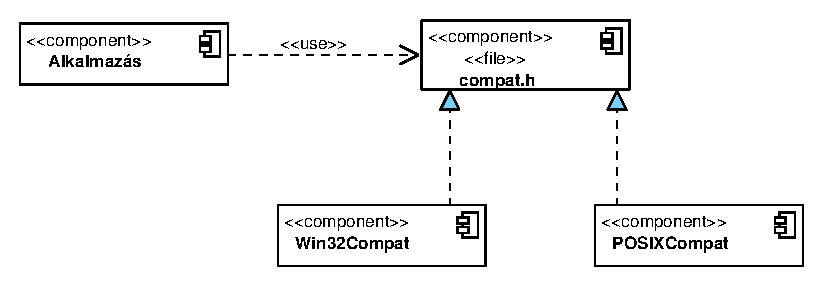
\includegraphics[width=.8\linewidth]{figures/compat.eps}
\caption{A kompatibilitási réteg felépítése}
\label{fig:compat}
\end{figure}

A blAST eszköz segítségével meg lehet adni, hogy a kompatibilitási rétegben definiált függvényeket konkrétan keresse meg, és jelentse az absztrakció fölött található alkalmazás kódjában.
Ez teljesen projekt specifikus ellenőrzés, így általános eszközökkel nem megvalósítható.
Viszont a blAST eszköz felhasználásával már fejlesztéskor futtatható lokális ellenőrzésként kiderülhet, hogy véletlenül direkt módon került meghívásra az operációs rendszer sajátos interfésze.

\section{Oktatás}

Egy nagyon jó példa a különböző programozást és a hozzá tartozó nyelveket tanító tárgyak számonkérései.
Szinte minden alapozó tárgy ilyen témakörben tartalmaz valamiféle megkötéseket, hogy a hallgatóságot a ,,jó szokások'' felé terelje.
Például, az informatikus képzés Programozás Alapjai 1 c.~tárgy (C) házi feladatában a globális változók használata tiltott, míg a Programozás Alapjai 2 tárgyban (C++) a típus lekérdezésekért járnak levonások.
Nyilván, mind két esetben sok más egyéb kritériumnak és minőségi elvárásnak is meg kell felelnie a kódnak.

Hasonlóan lehetséges, hogy egyes feladatok olyan anyagot kérnének számon, amelyiket magától lehetséges kikerülni másik nyelvi eszközökkel.
Például, ha a feladat arra kíváncsi, hogy a C++ szabványos könyvtár algoritmusait képes-e a hallgató használni, akkor a megoldást manuálisan megírni egy ciklussal nem jó válasz.
Ennek megfelelően lehetséges primitív szöveg alapú ellenőrzéseket csinálni, de például makrókkal ez könnyen kicselezhető.
Konkrét esetekre lehet reagálni, de az ilyen jellegű megoldások mindig is ki lesznek téve különböző cseles megoldásoknak, hogy a hallgató egy ciklust írhasson.

Az automatikusan javított feladatoknál pedig ez nem is lehetőség, de manuális ellenőrzések esetén, például a házi feladatnál, ezek a hibák nyilván kibuknak.
De emiatt szükséges nagyon alaposan átnézni a hallgatói kódokat, hiszen benne rejtőzhetnek az ilyen-olyan hibák.
A probléma, hogy egyes esetekben lehetséges, hogy a javító nem veszi észre.
Ezért hasznos lenne egy olyan eszköz, amelyik a könnyen ellenőrizhető hibás mintákat, vagy hibásnak vélt kódrészleteket, meg tudja keresni, és jelezni az oktató számára.

A másik előny származhat esetlegesen a hallgatók által való használatból is: ha van egy olyan program, amellyel a saját házifeladataik alapvető kritériumait tudják vizsgálni, azzal gyorsabb lesz a visszacsatolás, és lehetősége lehet olyan hibák javítására, amelyeket csak véletlen nem vett észre.
Ez csökkenti a terhet az oktatóról, és segíti a hallgatókat, hogy tudják javítani az egyértelműen hibás részeit a feladataiknak.

Ezekre a célokra mind nagyon jól használható a blAST eszköz.
A tárgyhoz tartozó kritériumokat fel lehetséges sorolni a számára egy forrásfájlban, és azt mindenki fel tudja használni, hogy a saját feladatát könnyítse, pontosítsa.
Az egyes automata kiértékelő rendszerekbe pedig lehetséges egy olyan lépést beépíteni, amelyikben lehetőség adódik a konkrét feladatok sajátosságait felülvizsgálni (\pl nincs ciklus a kódban).

Ezek egy része általános jó tanács, azonban nem olyan szinten általános, hogy be lennének építve a kulcsrakész rendszerekbe.
Emiatt a blAST eszköz rugalmassága nyújtja, a kényelmes használhatóságot mind az oktatói, mind a hallgatói oldalon.

